\begin{figure}[H]
   \centering
   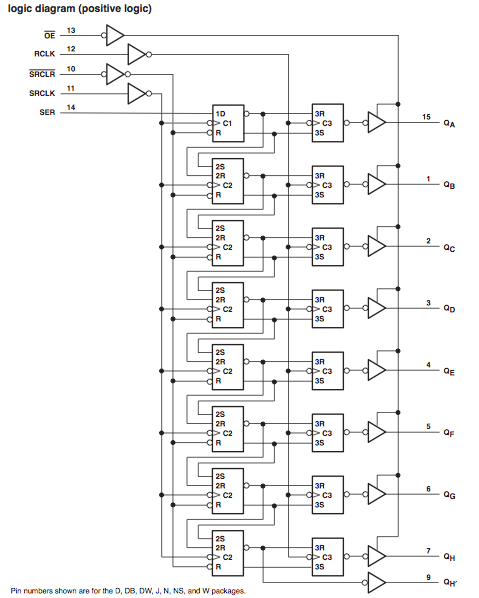
\includegraphics[width=0.5\textwidth]{img/Shift_register.png}%
   \caption{Shift register, source \url{http://www.ti.com/lit/ds/symlink/cd74hc595.pdf}}
   \label{fig:shiftRegister}%
\end{figure}


\begin{figure}[H]
   \centering
   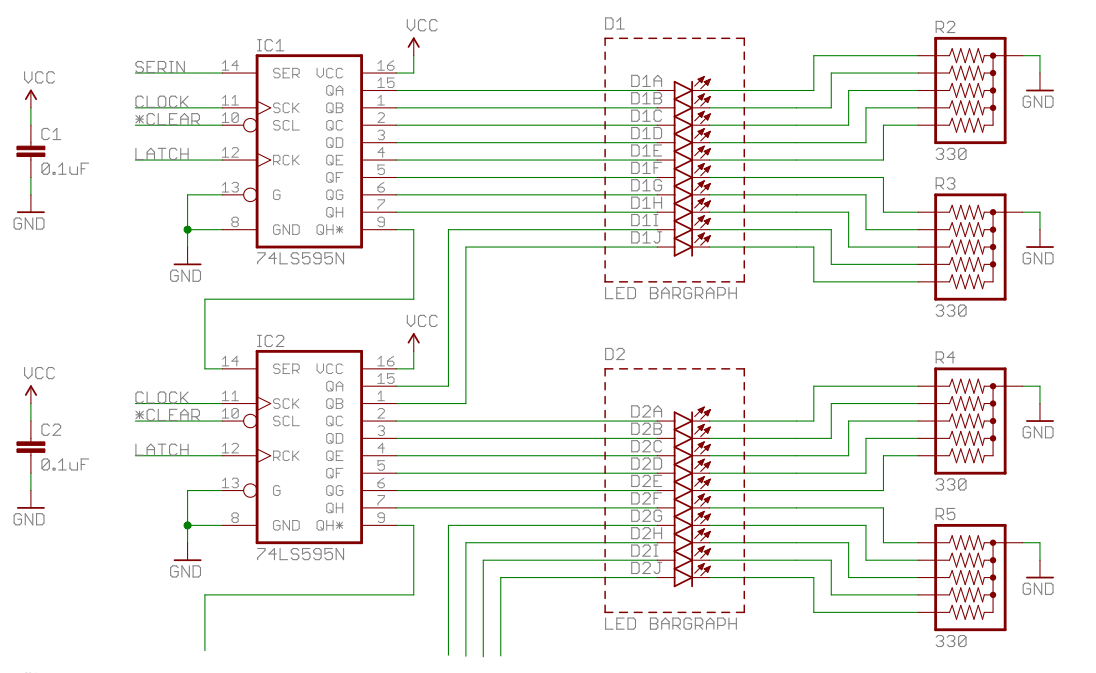
\includegraphics[width=0.8\textwidth]{img/Breakout.png}%
   \caption{Source \url{http://dlnmh9ip6v2uc.cloudfront.net/datasheets/BreakoutBoards/Bargraph Breakout v10.pdf}}
   \label{fig:breakout}%
\end{figure}


\begin{figure}[H]
   \centering
   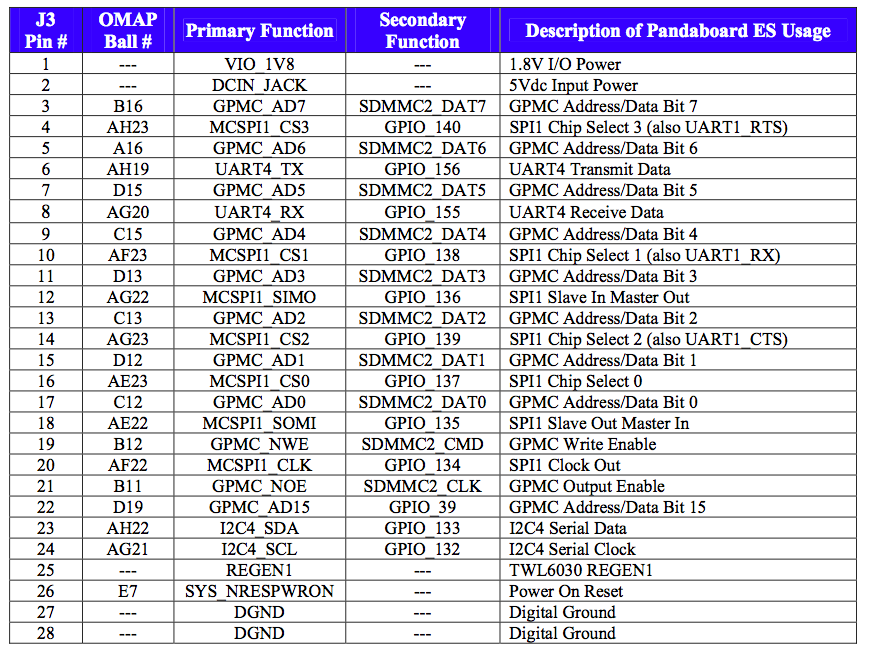
\includegraphics[width=0.8\textwidth]{img/PandaBoard_IO_J3.png}%
   \caption{Pandaboard IO J3 connectors,  source  \url{http://pandaboard.org/sites/default/files/board_reference/ES/Panda_Board_Spec_DOC-21054_REV0_1.pdf}}
   \label{fig:pandaBoardIOJ3}%
\end{figure}


\begin{table}[h]
\centering
\begin{tabular}{| l |  p{7cm} |}
\hline
\textbf{Pin} & \textbf{Used for} \\ \hline
1 & 1.8 Volt Referenz für level Shifter \\ \hline
2 & 5 Volt für Shift Register, LEDs und level shifter. \\ \hline
4 & GPIO 140 für Latch signal. \\ \hline
12 & SPI 1 Slave in Master out  für seriellen Datenstrom \\ \hline
20 & SPI 1 clock für shift Register Takt signal \\ \hline
27 & GND \\ \hline
28 & GND \\
\hline
\end{tabular}
\caption{Used J3 pins for this project}
\label{tab:pinUsageTable}
\end{table}


\begin{figure}[H]
   \centering
   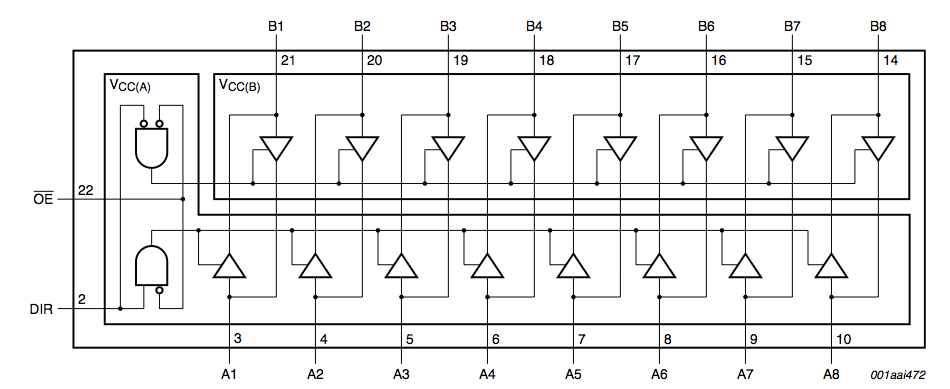
\includegraphics[width=0.8\textwidth]{img/level_Shifter.png}%
   \caption{Level shifter, source NXP  74LVC8T245 Manual}
   \label{fig:level_Shifter}%
\end{figure}

\begin{figure}[H]
   \centering
   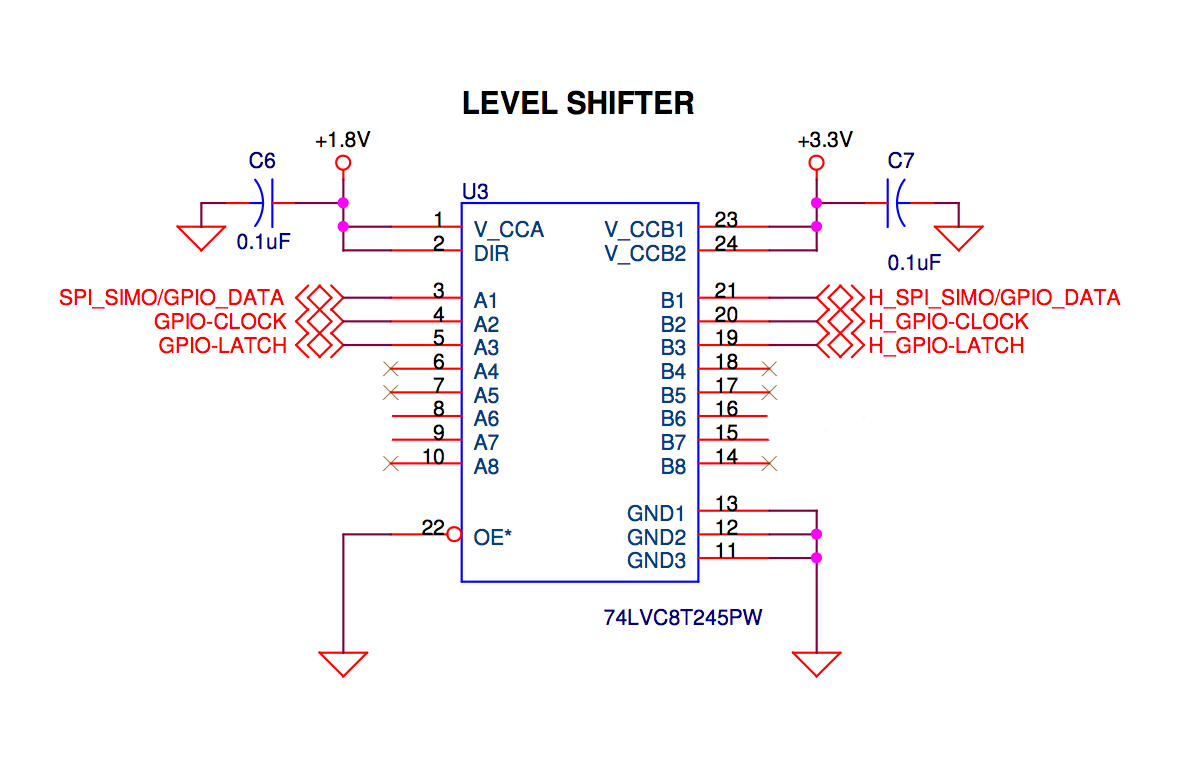
\includegraphics[width=0.8\textwidth]{img/Levelshifter.png}%
   \caption{Level Shifter, source: \url{http://www.tincantools.com/assets/BEACON REV-B .pdf}}
   \label{fig:levelShifter2}%
\end{figure}